%!TEX root = ../DigSig2.tex

%%%%%%%%%%%%%%%%%%%%%%%%%%%%%%%%%%%%%%%%%%%%%%%%%%%%%%%%%%%%
\section{FIR Digital Filter Design\buch{Chapter 10}}

%%%%%%%%%%%%%%%%%%%%%%%%%%%%%%%%%%%%%%%%%%%%%%%%%%%%%%%%%%%%
\subsection{Window Method\buchSeite{532-541}}

%%%%%%%%%%%%%%%%%%%%%%%%%%%%%%%%%%%%%%%%%%%%%%%%%%%%%%%%%%%%
\subsubsection{Ideal Filters\buchSeite{532-534}}

The design of an FIR filter using the window method starts from an ideal
frequency response $D(\omega)$. Since ideal filters are non-causal and
have an infinite impulse response, they cannot be implemented directly.
Therefore, the infinite impulse response is truncated by applying a
window function.

The ideal frequency response and its corresponding impulse response are
related by the inverse DTFT

\begin{equation}
d(k)=\int_{-\pi}^{\pi}
D(\omega)e^{j\omega k}
\frac{d\omega}{2\pi}
\label{eq:impresp}
\end{equation}

%%%%%%%%%%%%%%%%%%%%%%%%%%%%%%%%%%%%%%%%%%%%%%%%%%%%%%%%%%%%

\begin{figure}[htp]

\begin{subfigure}{0.49\textwidth}
\centering
\newcommand{\coordinates}{coordinates {
(-3.14,1) (-1.569,1) (-1.571,0)
(1.571,0) (1.569,1) (3.14,1)
};}
\input{tikz/hplp.tex}
\caption{Highpass\\[2mm]
$\displaystyle
D(\omega)=
\begin{cases}
1,&|\omega|>\omega_c\\
0,&|\omega|\le\omega_c
\end{cases}
$
}
\end{subfigure}
\begin{subfigure}{0.49\textwidth}
\centering
\newcommand{\coordinates}{coordinates {
(-3.14,0) (-1.569,0) (-1.571,1)
(1.571,1) (1.569,0) (3.14,0)
};}
\input{tikz/hplp.tex}
\caption{Lowpass\\[2mm]
$\displaystyle
D(\omega)=
\begin{cases}
1,&|\omega|\le\omega_c\\
0,&|\omega|>\omega_c
\end{cases}
$
}
\end{subfigure}

\begin{subfigure}{0.49\textwidth}
\centering
\newcommand{\coordinates}{coordinates {
(-3.14,1) (-2.001,1) (-1.999,0)
(-1.001,0) (-0.999,1)
(0.999,1) (1.001,0)
(1.999,0) (2.001,1) (3.14,1)
};}
\input{tikz/bpbs.tex}
\caption{Bandstop\\[2mm]
$\displaystyle
D(\omega)=
\begin{cases}
0,&\omega_a<|\omega|<\omega_b\\
1,&\text{otherwise}
\end{cases}
$
}
\end{subfigure}
\begin{subfigure}{0.49\textwidth}
\centering
\newcommand{\coordinates}{coordinates {
(-3.14,0) (-2.001,0) (-1.999,1)
(-1.001,1) (-0.999,0)
(0.999,0) (1.001,1)
(1.999,1) (2.001,0) (3.14,0)
};}
\input{tikz/bpbs.tex}
\caption{Bandpass\\[2mm]
$\displaystyle
D(\omega)=
\begin{cases}
1,&\omega_a<|\omega|<\omega_b\\
0,&\text{otherwise}
\end{cases}
$
}
\end{subfigure}

\begin{subfigure}{0.49\textwidth}
\centering
\newcommand{\coordinates}{coordinates {
(-3.14,-1) (3.14,1)
};}
\input{tikz/diffhilb.tex}
\caption{Differentiator\\[2mm]
$\displaystyle D(\omega)=j\omega$
}
\end{subfigure}
\begin{subfigure}{0.49\textwidth}
\centering
\newcommand{\coordinates}{coordinates {
(-3.14,1) (-0.001,1)
(0.001,-1) (3.14,-1)
};}
\input{tikz/diffhilb.tex}
\caption{Hilbert transformer\\[2mm]
$\displaystyle D(\omega)=-j\,\mathrm{sign}(\omega)$
}
\end{subfigure}

\caption{Ideal desired frequency responses $D(\omega)$\buchSeite{533}}
\label{fig:freqresp}

\end{figure}

%%%%%%%%%%%%%%%%%%%%%%%%%%%%%%%%%%%%%%%%%%%%%%%%%%%%%%%%%%%%

For the most common ideal filters, the impulse responses are

\begin{align*}
\text{Lowpass} \qquad
d(k)
&=
\frac{\sin(\omega_ck)}
{\pi k}
\\[1ex]
\text{Highpass} \qquad
d(k)
&=
\delta(k)
-
\frac{\sin(\omega_ck)}
{\pi k}
\\[1ex]
\text{Bandpass} \qquad
d(k)
&=
\frac
{\sin(\omega_bk)-\sin(\omega_ak)}
{\pi k}
\\[1ex]
\text{Bandstop} \qquad
d(k)
&=
\delta(k)
-
\frac
{\sin(\omega_bk)-\sin(\omega_ak)}
{\pi k}
\\[1ex]
\text{Differentiator} \qquad
d(k)
&=
\frac{\cos(\pi k)}{k}
-
\frac{\sin(\pi k)}
{\pi k^2}
\\[1ex]
\text{Hilbert transformer} \qquad
d(k)
&=
\frac{1-\cos(\pi k)}
{\pi k}
\end{align*}

For

\[
k=0
\]

the corresponding limits have to be evaluated separately.

%%%%%%%%%%%%%%%%%%%%%%%%%%%%%%%%%%%%%%%%%%%%%%%%%%%%%%%%%%%%
\subsubsection{FIR Filter Properties}

\paragraph{Complementary Filters}

\begin{align*}
d_{LP}(k)+d_{HP}(k)&=\delta(k)
&
\Longleftrightarrow
&
D_{LP}(\omega)+D_{HP}(\omega)=1
\\
d_{BP}(k)+d_{BS}(k)&=\delta(k)
&
\Longleftrightarrow
&
D_{BP}(\omega)+D_{BS}(\omega)=1
\end{align*}

%%%%%%%%%%%%%%%%%%%%%%%%%%%%%%%%%%%%%%%%%%%%%%%%%%%%%%%%%%%%

\paragraph{Symmetry}

\begin{center}
\renewcommand{\arraystretch}{1.2}
\begin{tabular}{l|c|c}
& Symmetric & Antisymmetric\\
\hline
Impulse response
&
$d(k)=d(-k)$
&
$d(k)=-d(-k)$
\\

Examples
&
LP, HP, BP, BS
&
Differentiator, Hilbert
\\

Frequency response
&
real, even
&
imaginary, odd
\\

Phase
&
linear
&
linear
\end{tabular}
\end{center}

%%%%%%%%%%%%%%%%%%%%%%%%%%%%%%%%%%%%%%%%%%%%%%%%%%%%%%%%%%%%

\paragraph{FIR Implementation}

\[
\boxed{
y(n)=
\sum_{m=0}^{N-1}
h(m)x(n-m)
}
\]

\begin{center}
\begin{tabular}{ll}
$h(m)$ & FIR coefficients\\
$x(n)$ & input\\
$y(n)$ & output\\
$N$ & filter length
\end{tabular}
\end{center}

%%%%%%%%%%%%%%%%%%%%%%%%%%%%%%%%%%%%%%%%%%%%%%%%%%%%%%%%%%%%

\paragraph{Group Delay}

For a linear-phase FIR filter

\[
\boxed{
\tau_g=\frac{N-1}{2}
\text{ samples}
}
\]

or

\[
\boxed{
t_g=\frac{N-1}{2f_s}
}
\]

where $N$ is the filter length and $f_s$ the sampling frequency.

%%%%%%%%%%%%%%%%%%%%%%%%%%%%%%%%%%%%%%%%%%%%%%%%%%%%%%%%%%%%
\subsubsection{Window Comparison}

The most common window functions differ mainly in

\begin{itemize}
\item transition width,
\item stopband attenuation,
\item passband ripple,
\item sidelobe attenuation.
\end{itemize}

\begin{center}
\renewcommand{\arraystretch}{1.25}
\begin{tabular}{|l|c|c|c|c|c|c|}
\hline
Window &
$\delta$ &
$A_{stop}$ &
$A_{pass}$ &
$D$ &
$R$ &
$c$
\\
\hline

Rectangular
&
$8.9\%$
&
$-21$ dB
&
$1.55$ dB
&
0.922
&
$-13$ dB
&
1
\\
\hline

Hamming
&
$0.2\%$
&
$-54$ dB
&
$0.03$ dB
&
3.21
&
$-40$ dB
&
2
\\
\hline

Kaiser
&
variable
&
$-20\log_{10}\delta$
&
$17.372\,\delta$
&
$
\begin{cases}
\dfrac{A-7.95}{14.36},
&A>21
\\[1ex]
0.922,
&A\le21
\end{cases}
$
&
variable
&
$\dfrac{6(R+12)}{55}$
\\
\hline

\end{tabular}
\end{center}

\subsubsection{Rectangular Window\buchSeite{535}}
\begin{multicols}{2}
	\begin{itemize}
		\item Simplest window, Length $N = 2M+1$
		\item truncate the infinite impulse response: \\ $-M \leq k \leq M$
		\item $\rightarrow \mathbf{d} = [d_{-M}, ..., d_{-1}, d_0, d_1, ..., d_M]$
		\item The resulting causal FIR Filter must be delayed by M samples \newline
		$\rightarrow \mathbf{h} = \mathbf{d} = [h_0, h_{M-1}, h_M, h_{M+1}, ..., h_{2M}]$
	\end{itemize}

	\begin{center}
		\input{tikz/rectwindow.tex}
	\end{center}
\end{multicols}


%%%%%%%%%%%%%%%%%%%%%%%%%%%%%%%%%%%%%%%%%%%%%%%%%%%%%%%%%%%%
\paragraph{Gibbs Phenomenon}

Truncating the infinite impulse response introduces oscillations close
to the cutoff frequency.

Characteristics:

\begin{itemize}
\item Overshoot approximately $8.9\%$
\item Independent of the filter length
\item Increasing $N$ narrows the oscillation region
\item The oscillation amplitude does not disappear
\end{itemize}

\subsubsection{Hamming Window\buchSeite{540}}
\begin{itemize}
	\item Improved passband and stopband ripple suppression at the cost of a wider transition width.
	\item Hamming window impulse response:
	\begin{align*}
		w(n) = 0.54 -0.46\cos\left(\frac{2\pi n}{N-1}\right),&&n= 0,1,\dots,N-1
	\end{align*}
	\item Filter impuls response:
	\begin{align*}
		h(n) = w(n)d(n-M),&&-\infty < n < \infty
	\end{align*}
	\item e.g. lowpass filter
	\begin{align*}
		h(n) = \left[0.54 -0.46\cos\left(\frac{2\pi n}{N-1}\right)\right]\cdot\frac{\sin(\omega_c(n-M))}{\pi (n-M)}
	\end{align*}
\end{itemize}

\paragraph{Properties}

Compared to the rectangular window:

\begin{itemize}
\item much smaller passband ripple
\item much smaller stopband ripple
\item lower sidelobes
\item wider transition band
\item ripple approximately $0.2\%$
\end{itemize}

%%%%%%%%%%%%%%%%%%%%%%%%%%%%%%%%%%%%%%%%%%%%%%%%%%%%%%%%%%%%
\subsubsection{Hann Window}

The Hann window is defined by

\[
w(n)
=
0.5
-
0.5
\cos
\left(
\frac{2\pi n}{N-1}
\right),
\qquad
n=0,1,\ldots,N-1.
\]

Compared to the Hamming window, the Hann window provides slightly wider
main lobes but lower spectral leakage than the rectangular window.

%%%%%%%%%%%%%%%%%%%%%%%%%%%%%%%%%%%%%%%%%%%%%%%%%%%%%%%%%%%%
\subsubsection{Kaiser Window\buchSeite{541}}

The Kaiser window is a family of window functions whose shape can be
adjusted by the parameter $\alpha$.

Unlike the rectangular and Hamming windows, the Kaiser window allows a
trade-off between

\begin{itemize}
\item transition width,
\item stopband attenuation,
\item filter length.
\end{itemize}

\vspace{0.5em}

\begin{center}
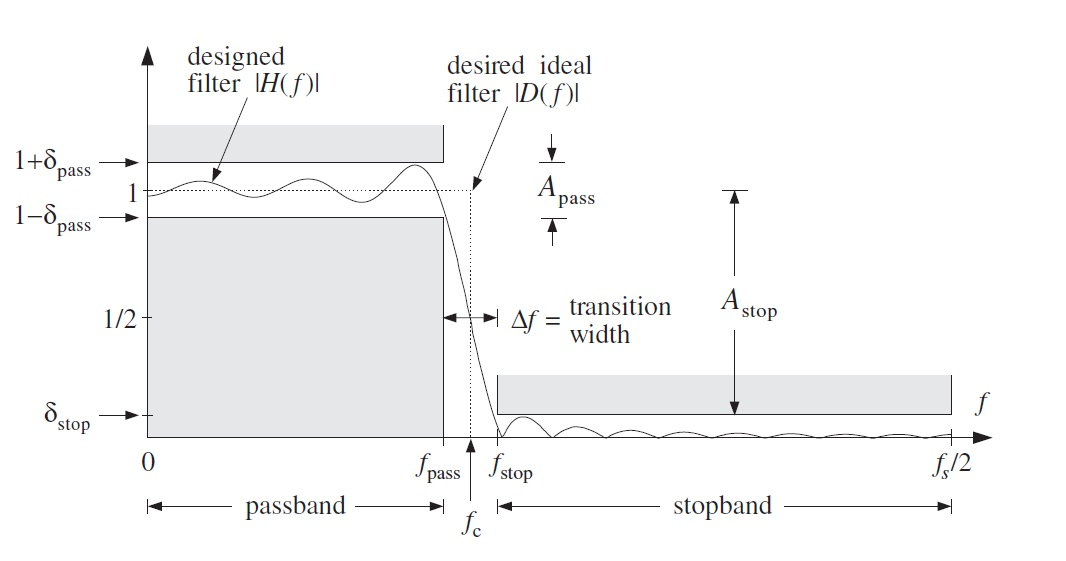
\includegraphics[width=10cm]{images/FIR_KaiserSpecs.jpg}
\end{center}

\vspace{0.5em}

\renewcommand{\arraystretch}{1.3}

\begin{center}
\begin{tabular}{|l|l|}
\hline

Cutoff frequency
&
$
f_c
=
\frac12
(f_{pass}+f_{stop})
$
\\
\hline

Transition width
&
$
\Delta f
=
f_{stop}-f_{pass}
$
\\
\hline

Passband / Stopband frequencies
&
$
f_{pass}
=
f_c-\frac{\Delta f}{2},
\qquad
f_{stop}
=
f_c+\frac{\Delta f}{2}
$
\\
\hline

Digital frequencies
&
$
\omega_{pass}
=
\frac{2\pi f_{pass}}{f_s},
\qquad
\omega_{stop}
=
\frac{2\pi f_{stop}}{f_s}
$
\\

&
$
\omega_c
=
\frac{2\pi f_c}{f_s},
\qquad
\Delta\omega
=
\frac{2\pi\Delta f}{f_s}
$
\\
\hline

Passband / Stopband ripple
&
$
A_{pass}
=
20\log_{10}
\left(
\frac{1+\delta_{pass}}
{1-\delta_{pass}}
\right)
$
\\

&
$
A_{stop}
=
-20\log_{10}
(\delta_{stop})
$
\\

&
$
\delta_{pass}
=
\frac
{10^{A_{pass}/20}-1}
{10^{A_{pass}/20}+1}
$
\\

&
$
\delta_{stop}
=
10^{-A_{stop}/20}
$
\\
\hline

Window parameters
&
$
\alpha=
\begin{cases}
0.1102(A-8.7),
&
A\ge50
\\
0.5842(A-21)^{0.4}
+
0.07886(A-21),
&
21<A<50
\\
0,
&
A\le21
\end{cases}
$
\\

&
$
D=
\begin{cases}
\dfrac{A-7.95}{14.36},
&
A>21
\\
0.922,
&
A\le21
\end{cases}
$
\\
\hline

Window function
&
$
w(n)
=
\frac
{
I_0
\left(
\alpha
\sqrt{
1-
\dfrac{(n-M)^2}{M^2}
}
\right)
}
{I_0(\alpha)}
$
\\

&
$
=
\frac
{
I_0
\left(
\dfrac
{\alpha\sqrt{n(2M-n)}}
{M}
\right)
}
{I_0(\alpha)}
$
\\

&
$
I_0
=
\text{modified Bessel function of first kind, order }0
$
\\

\hline
\end{tabular}
\end{center}

%%%%%%%%%%%%%%%%%%%%%%%%%%%%%%%%%%%%%%%%%%%%%%%%%%%%%%%%%%%%
\paragraph{Lowpass Design (Kaiser Window)\buchSeite{544}}

\begin{enumerate}
\item Cutoff and transition width
\[
f_c=\frac{f_{pass}+f_{stop}}{2},
\qquad
\Delta f=f_{stop}-f_{pass}
\]

\item Digital cutoff frequency
\[
\omega_c=\frac{2\pi f_c}{f_s}
\]

\item Passband and stopband ripples
\[
\delta_{pass}=
\frac{10^{A_{pass}/20}-1}
{10^{A_{pass}/20}+1},
\qquad
\delta_{stop}=10^{-A_{stop}/20}
\]

\item Select the smaller ripple
\[
\delta=\min(\delta_{pass},\delta_{stop}),
\qquad
A=-20\log_{10}\delta
\]

(Kaiser uses the smaller ripple.)

\item Calculate the Kaiser parameters
\[
\alpha,\qquad D
\]

\item Filter length
\[
N=\frac{Df_s}{\Delta f}+1
\]

Round $N$ up to the next odd integer and calculate

\[
M=\frac{N-1}{2}.
\]

\item Kaiser window
\[
w(n),\qquad n=0,\ldots,N-1
\]

\item FIR coefficients
\[
h(n)=w(n)d(n-M)
\]

\end{enumerate}

%%%%%%%%%%%%%%%%%%%%%%%%%%%%%%%%%%%%%%%%%%%%%%%%%%%%%%%%%%%%
\subsubsection{Kaiser Design Equations}

For a Kaiser window design the transition bandwidth and the filter
length are approximately related by

\[
\boxed{
N
\approx
\frac{D}{\Delta F}
}
\]

where

\[
\Delta F
=
\frac{\Delta f}{f_s}
\]

is the normalized transition width.

The transition width is

\[
\boxed{
\Delta f
=
f_{stop}-f_{pass}
}
\]

The cutoff frequency is

\[
\boxed{
f_c
=
\frac{f_{pass}+f_{stop}}2
}
\]

or, in digital frequency,

\[
\boxed{
\omega_c
=
2\pi
\frac{f_c}{f_s}.
}
\]

%%%%%%%%%%%%%%%%%%%%%%%%%%%%%%%%%%%%%%%%%%%%%%%%%%%%%%%%%%%%
\subsubsection{Implementation Limits}

For real-time DSP implementations, the maximum filter length is limited
by the available instruction rate.

\[
\boxed{
N_{\max}
\approx
\frac{f_{\mathrm{instr}}}{f_s}
}
\]

where

\begin{itemize}
\item $f_{\mathrm{instr}}$ is the DSP instruction rate,
\item $f_s$ is the sampling frequency.
\end{itemize}

The corresponding minimum transition bandwidth is

\[
\boxed{
\Delta f_{\min}
=
\frac
{Df_s^2}
{f_{\mathrm{instr}}}
}
\]

where $D$ is the Kaiser design parameter.

%%%%%%%%%%%%%%%%%%%%%%%%%%%%%%%%%%%%%%%%%%%%%%%%%%%%%%%%%%%%
\paragraph{Maximum Achievable Stopband Attenuation}

For a fixed DSP instruction rate the maximum achievable attenuation is

\[
\boxed{
A_{\max}
=
14.36
F_{\mathrm{instr}}
\Delta F
+
7.95
}
\]

with

\[
F_{\mathrm{instr}}
=
\frac{f_{\mathrm{instr}}}{f_s},
\qquad
\Delta F
=
\frac{\Delta f}{f_s}.
\]

%%%%%%%%%%%%%%%%%%%%%%%%%%%%%%%%%%%%%%%%%%%%%%%%%%%%%%%%%%%%
\subsubsection{Rules for Different Filter Types}

\paragraph{Highpass Filter}

For a highpass filter, the passband and stopband are exchanged.

Therefore,

\[
\boxed{
\Delta f
=
f_{pass}-f_{stop}.
}
\]

%%%%%%%%%%%%%%%%%%%%%%%%%%%%%%%%%%%%%%%%%%%%%%%%%%%%%%%%%%%%
\paragraph{Bandpass Filter}

\begin{center}
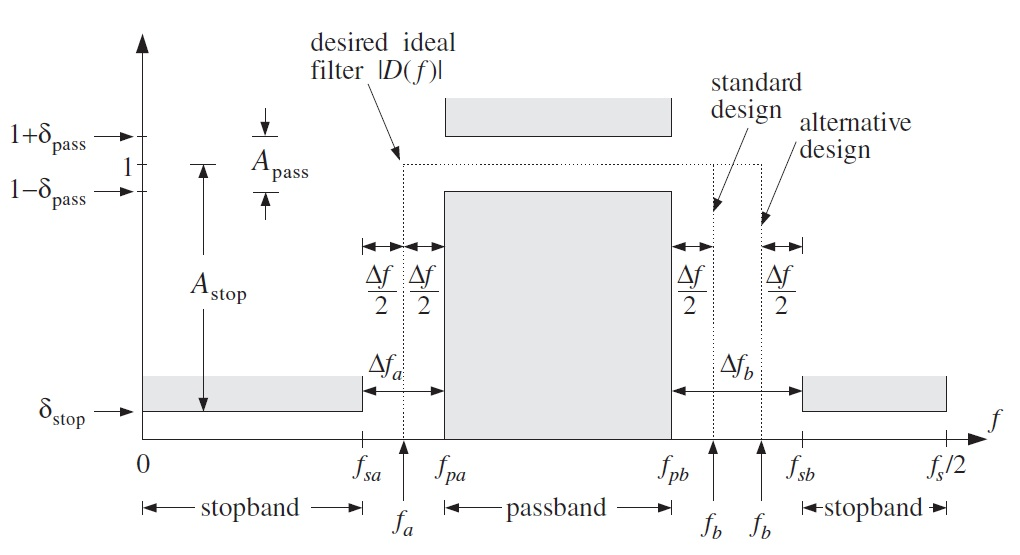
\includegraphics[width=8cm]{images/FIR_KaiserBP.jpg}
\end{center}

The final filter has equal transition widths

\[
\boxed{
\Delta f
=
\min(\Delta f_a,\Delta f_b)
}
\]

with

\[
\Delta f_a
=
f_{pa}-f_{sa},
\]

\[
\Delta f_b
=
f_{sb}-f_{pb}.
\]

Two design choices are possible.

\paragraph{Focus on Passband}

\[
f_a
=
f_{pa}
-
\frac{\Delta f}{2},
\]

\[
f_b
=
f_{pb}
+
\frac{\Delta f}{2}.
\]

\paragraph{Focus on Stopband}

\[
f_a
=
f_{sa}
+
\frac{\Delta f}{2},
\]

\[
f_b
=
f_{sb}
-
\frac{\Delta f}{2}.
\]

%%%%%%%%%%%%%%%%%%%%%%%%%%%%%%%%%%%%%%%%%%%%%%%%%%%%%%%%%%%%
\subsubsection{Kaiser Window for Spectral Analysis\buchSeite{555}}

The Kaiser window can also be used for spectral analysis (DFT and FFT).

For a desired sidelobe level

\[
R
\]

the parameter

\[
c
\]

is calculated as

\[
\boxed{
c
=
\frac{6(R+12)}{155}
}
\]

The corresponding Kaiser shape parameter is

\[
\alpha
=
\begin{cases}
0,
&
R<13.26
\\[1ex]
0.76609(R-13.26)^{0.4}
+
0.09834(R-13.26),
&
13.26<R<60
\\[1ex]
0.12438(R+6.3),
&
60<R<120.
\end{cases}
\]

%%%%%%%%%%%%%%%%%%%%%%%%%%%%%%%%%%%%%%%%%%%%%%%%%%%%%%%%%%%%
\subsection{Frequency Sampling Method\buchSeite{558}}

For an arbitrary frequency response

\[
D(\omega),
\]

the inverse DTFT generally cannot be evaluated analytically. Therefore,
the impulse response is approximated by sampling the desired frequency
response at equally spaced frequencies.

Instead of

\[
d(k)
=
\int_{-\pi}^{\pi}
D(\omega)e^{j\omega k}
\frac{d\omega}{2\pi},
\]

the approximation

\[
\boxed{
\tilde d(k)
=
\frac1N
\sum_{i=-M}^{M}
D(\omega_i)
e^{j\omega_i k}
}
\]

is used, where

\[
-M\le k\le M.
\]

If

\[
N=2M+1,
\]

the approximation corresponds to an inverse

\[
N\text{-point DFT}.
\]

%%%%%%%%%%%%%%%%%%%%%%%%%%%%%%%%%%%%%%%%%%%%%%%%%%%%%%%%%%%%

\paragraph{Windowing}

As with the Window Method, the sampled impulse response is multiplied by
a window function.

\[
\boxed{
h(n)
=
w(n)\,
\tilde d(n-M),
\qquad
n=0,1,\ldots,N-1.
}
\]

Therefore, every window introduced previously (Rectangular, Hamming,
Kaiser, ...) can also be used together with the Frequency Sampling
Method.

%%%%%%%%%%%%%%%%%%%%%%%%%%%%%%%%%%%%%%%%%%%%%%%%%%%%%%%%%%%%
\paragraph{Design Procedure}

The Frequency Sampling Method consists of the following steps:

\begin{enumerate}
\item Specify the desired frequency response
      $D(\omega)$.

\item Sample the frequency response at
      equally spaced frequencies.

\item Perform an inverse DFT to obtain
      the impulse response.

\item Apply a suitable window function.

\item Shift the impulse response by
      $M=(N-1)/2$
      samples to obtain a causal FIR filter.
\end{enumerate}

%%%%%%%%%%%%%%%%%%%%%%%%%%%%%%%%%%%%%%%%%%%%%%%%%%%%%%%%%%%%
\paragraph{Comparison with the Window Method}

\begin{center}
\renewcommand{\arraystretch}{1.25}
\begin{tabular}{|p{6cm}|p{6cm}|}
\hline
\textbf{Window Method}
&
\textbf{Frequency Sampling Method}
\\
\hline

Starts from an analytical ideal response
&
Starts from discrete frequency samples
\\
\hline

Requires inverse DTFT
&
Requires inverse DFT
\\
\hline

Simple for standard filters
&
Suitable for arbitrary frequency responses
\\
\hline

Window applied after truncation
&
Window applied after IDFT
\\
\hline

\end{tabular}
\end{center}

%%%%%%%%%%%%%%%%%%%%%%%%%%%%%%%%%%%%%%%%%%%%%%%%%%%%%%%%%%%%
\subsection{Other FIR Design Methods\buchSeite{558}}

Although the Kaiser Window Method is simple and flexible, other FIR
design techniques often achieve a better approximation with shorter
filters.

The most important alternative is the

\[
\boxed{\text{Parks--McClellan Algorithm}}
\]

which is based on the

\[
\boxed{\text{Equiripple Chebyshev Approximation}.}
\]

%%%%%%%%%%%%%%%%%%%%%%%%%%%%%%%%%%%%%%%%%%%%%%%%%%%%%%%%%%%%
\paragraph{Characteristics}

Compared with the Window Method,

\begin{itemize}
\item the passband and stopband ripples have equal height,
\item the approximation error is minimized,
\item shorter filters are often sufficient,
\item the design is computationally more involved.
\end{itemize}

%%%%%%%%%%%%%%%%%%%%%%%%%%%%%%%%%%%%%%%%%%%%%%%%%%%%%%%%%%%%
\paragraph{Comparison}

\begin{center}
\renewcommand{\arraystretch}{1.25}
\begin{tabular}{|p{6cm}|p{6cm}|}
\hline
\textbf{Window Method}
&
\textbf{Parks--McClellan}
\\
\hline

Simple design
&
Optimal design
\\
\hline

Longer filters
&
Shorter filters
\\
\hline

Window dependent
&
Equiripple approximation
\\
\hline

Very easy to implement
&
Iterative optimisation
\\
\hline

\end{tabular}
\end{center}
\newpage